\section{Activation of RTK}

The \SBGNERLone language is designed with so called ``open world assumption'' in mind. This means that all entities, state variables and interactions assumed to be independent, unless explicitly specified with influence arc. That approach helps to avoid combinatorial explosion and makes drawing of the diagram much easier compared to \SBGNPDLone, but it makes reading and analysis of the diagram more difficult and laborious.  

To illustrate creation and analysis of \SBGNERLone diagram we will create the diagram of receptor tyrosine kinase (RTK) activation pathway in a step by step manner. Wikipedia (\url{https://en.wikipedia.org/wiki/Receptor_tyrosine_kinase}) describes the process of RTK activation as follows:
\begin{quote}
``When a growth factor binds to the extracellular domain of an RTK, its dimerization is triggered with other adjacent RTKs. Dimerization leads to a rapid activation of the protein's cytoplasmic kinase domains, the first substrate for these domains being the receptor itself. The activated receptor as a result then becomes autophosphorylated on multiple specific intracellular tyrosine residues.''
\end{quote}

Drawing \SBGNERLone the diagram is simple, we will follow the textual description of the pathway and add required elements. Let's start with identification of key players of the pathway. In a text we can figure out that two main entities are ``RTK'' and ``growth factor''. We will draw them as ``receptor'' and ``ligand''  entities (\sect{entity}) respectively. We could also notice that RTK has two domains: the ``extracellular domain'' (``receptor'') and the ``kinase domain'', they will also be shown in \fig{rtk-entities}. The pathway description also mentions ``multiple specific intracellular tyrosine residues'', so we've added two state variables (\sect{stateVariable}) ``Y1'' and ``Y2''' to the receptor entity to be able to show events related to modification of tyrosine residues.  

\begin{figure}[H]
  \centering
  \vspace*{-0.75em}
  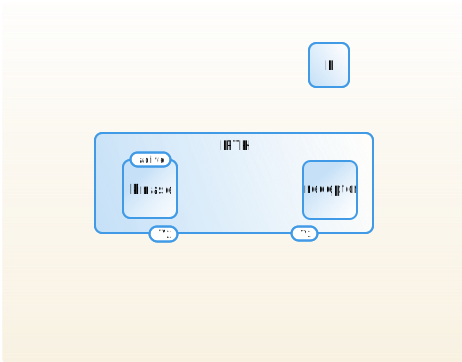
\includegraphics[scale=0.75]{examples/rtk-entities.png}
   \caption{Receptor tyrosine kinase activation: entities definition.}
  \label{fig:rtk-entities}
\end{figure}

By creation of entities we have populated our system with instances of two kinds: a ``receptor'' and a ``ligand''. We show also the internal structure of a receptor by depicting its two domains as nested entities (\sect{domain}). Receptor and its ``kinase'' domain carry out the ``state variable'' (\sect{stateVariable}) to define the basis of the entity state space.

The next step is to describe the part of entities state space we are going to be interested in. Two assignment arcs (\sect{assignment}) pointing to the ``Y1'' and ``Y2'' receptor state variables on figure \fig{rtk-states} demonstrate that we are going to analyse phosphorylation of tyrosine residues. We need also to take into account that according to the description ``Dimerization leads to a rapid activation of the protein's cytoplasmic kinase domains'', that means that the ``active'' state variable of ``kinase'' domain could become ``true'' after some perturbations in the system. So we've added an appropriate variable value (\sect{variableValue}) node and an assignment arc.

\SBGNERLone is a so called ``open world'' language, which means that as diagram developers we are not obliged to describe the whole system, we can leave unknown parts unaddressed and focus on the most important parts of the system. That's why we included only ``P'' state value for those residues. To describe the whole system we ought include ``unphosphorylate'' or some other ``default'' value as well (see \sect{assignment} to check how to do it properly), but in our case it is not important so we'll use ``open world'' assumption and omit it.  \SBGNERLone assumes that all interactions are internally reversible, so even if we describe only the switch from default to phosphorylated state explicitly, that description implies that there is a mechanism to put ``Y1'' and ``Y2'' variables back to their default state. For the same reason we haven't added ``false'' value to the ``active'' state of the kinase domain.
 
\begin{figure}[H]
  \centering
  \vspace*{-0.75em}
  \includegraphics[scale=0.75]{examples/rtk-states.png}
   \caption{Receptor tyrosine kinase activation: state variable assignment.}
  \label{fig:rtk-states}
\end{figure}

By now we have prepared all elements that are taking part in the process description, and we are ready to draw the pathway itself. The first sentence of the pathway description starts with ``When a growth factor \textbf{binds} to the extracellular domain of an RTK'', so the first event we are going to draw is a receptor ligand binding (\fig{rtk-binding}). We will use an interaction arc (\sect{interaction}) to show that the ligand can bind the receptor.

\begin{figure}[H]
  \centering
  \vspace*{-0.75em}
  \includegraphics[scale=0.75]{examples/rtk-binding.png}
   \caption{Receptor tyrosine kinase activation: receptor-ligand binding.}
  \label{fig:rtk-binding}
\end{figure}

The binding happens between the ligand entity and the receptor domain of the receptor entity. The interaction event is reversible in a same way as assignment. That means that even if two instances of ligand and receptor are bound at some time that bond will not last forever, it will dissociate with some probability.

Next step in the pathway is ``When a growth factor binds to the extracellular domain of an RTK, its \textbf{dimerization} is triggered with other adjacent RTKs''. The dimerisation event is added in \fig{rtk-dimerisation}. The interaction arc in that figure connects the entity with itself, so we need to distinguish two possibilities: receptor molecule binds another molecule of the same kind (what we need according to the pathway description) or it undergoes some intramolecular interaction. In the former case we add \glyph{unit of information} ``trans'' to the arc to emphasise that the interaction is intermolecular, the latter case would require \glyph{unit of information} ``cis'' (see \sect{unitInformation}, \sect{miscellaneous-cv} and \sect{cis-trans-semantics}). Definition of ``cis'' or ``trans'' interaction is meaningful only for events involving instances of the same entity, directly or via chain of events. If you do not specify cis/trans type of interaction it will be undefined, because of the ``open world'' nature of \SBGNERLone, which is absolutely legitimate and sometimes unavoidable choice, but the diagram is much more understandable if an \glyph{unit of information} of appropriate type is added to the interaction arc according to biological knowledge.

\begin{figure}[H]
  \centering
  \vspace*{-0.75em}
  \includegraphics[scale=0.75]{examples/rtk-dimerisation.png}
   \caption{Receptor tyrosine kinase activation: receptor dimer formation.}
  \label{fig:rtk-dimerisation}
\end{figure}

Now we have to emphasise that the dimerisation depends upon the ligand-receptor binding. There are two key elements of \SBGNERLone we are going to use in this step (see \fig{rtk-dimer-control}): outcome (\sect{outcome}) and influence arc (\sect{influences}). This is the first time we came across the need to use a result of interaction. In our case the result of interaction is a complex containing instances of receptor and ligand, but not limited to the binary complex, as we will see soon. To show the result of an interaction on the diagram the black dot is drawn on the interaction arc and this dot is the origin of our influence arc (\sect{influences}). Influence arcs are designed to depict the way one part of the system controls the behaviour of the other. The word ``triggered'' in a pathway description means that the interaction between receptor and ligand is necessary for the dimerisation process, so we've used necessary stimulation (\sect{necessaryStimulation}), which assumes that without the stimulator entity the target interaction would not take place. And we have placed ``cis'' \glyph{unit of information} on the influence arc to emphasise that the control happens within the same molecular complex. That means that the receptor-ligand complex is not the catalyst that forms a dimer from some other instances of receptor entity, instead the complex is always involves instance of a receptor that bound the ligand.
 
\begin{figure}[H]
  \centering
  \vspace*{-0.75em}
  \includegraphics[scale=0.75]{examples/rtk-dimer-control.png}
   \caption{Receptor tyrosine kinase activation: control of the dimer formation.}
  \label{fig:rtk-dimer-control}
\end{figure}

Following the next sentence in the pathway description, which says ``Dimerization leads to a rapid activation of the protein's cytoplasmic kinase domains,'' we are going to add another influence arc (see \fig{rtk-kinase-activation}), but this time the arc is a stimulation (\sect{stimulation}), which means that the kinase domain may be active to some extent even in monomeric form of a receptor. Again we have the outcome dot to represent the dimer, but in this case the outcome represents any kind of complex where two receptor molecules bound together.

\begin{figure}[H]
  \centering
  \vspace*{-0.75em}
  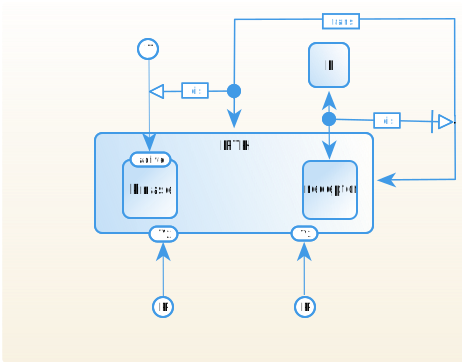
\includegraphics[scale=0.75]{examples/rtk-kinase-activation.png}
   \caption{Receptor tyrosine kinase activation: activation of the kinase domain of the receptor.}
  \label{fig:rtk-kinase-activation}
\end{figure}

The last and most important part of our pathway is the ``autophosphorylation of multiple specific intracellular tyrosine residues'' by activated kinase domain. The complete pathway is shown in \fig{rtk-full}. All interactions and influences in \SBGNERLone are independent, so for each stimulation arc representing autophosphorylation of the tyrosine residue we created their own outcome. Those outcomes represent independent sets of instances where kinase is active.

\begin{figure}[H]
  \centering
  \vspace*{-0.75em}
  \includegraphics[scale=0.75]{examples/rtk.png}
   \caption{The complete diagram of receptor tyrosine kinase activation.}
  \label{fig:rtk-full}
\end{figure}

Now, when our diagram is ready let's analyse it to get a better understanding of rules of the language and meaning of the diagram elements. The diagram consists of two types of entities, three types of outcomes, two interaction arcs, three assignment arcs, and four influence arcs. If we take into account independence and reversibility of all interactions we can count the total number of complexes that could be created in the system. It will be 153 complex types in total: 8 monomeric receptors, 8 monomeric receptor-ligand complexes, 36 receptor dimers, 64 receptor dimers with one ligand, 36 receptor dimers with two ligands and free ligand. Those numbers come from simple combinatorics, taking into account the number of state variables and assuming that each of them can have two values: ``undefined'' and specified by assignment arc. \fig{rtk-complexes} shows three of the 144 complexes compatible with the definition of outcome on the active kinase state assignment.

\begin{figure}[H]
  \centering
  \vspace*{-0.75em}
  \includegraphics[scale=0.75]{examples/rtk-complex.png}
   \caption{Receptor tyrosine kinase activation: examples of active kinase complexes are shown. Black lines connect two complexes with outcomes, which definition is compatible with the complex status.}
  \label{fig:rtk-complexes}
\end{figure}

That big number of possible complexes should not be scared of, because influence arcs in our model control the set of reachable states quite firmly. For example, blocking any phosphorylation sites reduces the number of reachable complexes to 45, and blocking kinase activation reduces the total set of possible complexes types to just 6. It could be easily seen from the diagram: in the former case we switch off one receptor state variable, in the later we effectively block all three: blocking activation assignment we render all its outcomes to false state. That means that activation will never happen and so tyrosine residues will never be phosporylated. Our diagram is quite simple, it does not contain any complex feed-backs, so results of analysis are rather trivial. The next sections show more complex and meaningful diagrams.
